% Font options: 10pm, 11pt, 12pt
% Align headings left instead of center: nocenter
\documentclass[xcolor=x11names,compress]{beamer}\usepackage[]{graphicx}\usepackage[]{color}
%% maxwidth is the original width if it is less than linewidth
%% otherwise use linewidth (to make sure the graphics do not exceed the margin)
\makeatletter
\def\maxwidth{ %
  \ifdim\Gin@nat@width>\linewidth
    \linewidth
  \else
    \Gin@nat@width
  \fi
}
\makeatother

\definecolor{fgcolor}{rgb}{0.345, 0.345, 0.345}
\newcommand{\hlnum}[1]{\textcolor[rgb]{0.686,0.059,0.569}{#1}}%
\newcommand{\hlstr}[1]{\textcolor[rgb]{0.192,0.494,0.8}{#1}}%
\newcommand{\hlcom}[1]{\textcolor[rgb]{0.678,0.584,0.686}{\textit{#1}}}%
\newcommand{\hlopt}[1]{\textcolor[rgb]{0,0,0}{#1}}%
\newcommand{\hlstd}[1]{\textcolor[rgb]{0.345,0.345,0.345}{#1}}%
\newcommand{\hlkwa}[1]{\textcolor[rgb]{0.161,0.373,0.58}{\textbf{#1}}}%
\newcommand{\hlkwb}[1]{\textcolor[rgb]{0.69,0.353,0.396}{#1}}%
\newcommand{\hlkwc}[1]{\textcolor[rgb]{0.333,0.667,0.333}{#1}}%
\newcommand{\hlkwd}[1]{\textcolor[rgb]{0.737,0.353,0.396}{\textbf{#1}}}%
\let\hlipl\hlkwb

\usepackage{framed}
\makeatletter
\newenvironment{kframe}{%
 \def\at@end@of@kframe{}%
 \ifinner\ifhmode%
  \def\at@end@of@kframe{\end{minipage}}%
  \begin{minipage}{\columnwidth}%
 \fi\fi%
 \def\FrameCommand##1{\hskip\@totalleftmargin \hskip-\fboxsep
 \colorbox{shadecolor}{##1}\hskip-\fboxsep
     % There is no \\@totalrightmargin, so:
     \hskip-\linewidth \hskip-\@totalleftmargin \hskip\columnwidth}%
 \MakeFramed {\advance\hsize-\width
   \@totalleftmargin\z@ \linewidth\hsize
   \@setminipage}}%
 {\par\unskip\endMakeFramed%
 \at@end@of@kframe}
\makeatother

\definecolor{shadecolor}{rgb}{.97, .97, .97}
\definecolor{messagecolor}{rgb}{0, 0, 0}
\definecolor{warningcolor}{rgb}{1, 0, 1}
\definecolor{errorcolor}{rgb}{1, 0, 0}
\newenvironment{knitrout}{}{} % an empty environment to be redefined in TeX

\usepackage{alltt}
%\documentclass[xcolor=x11names,compress,handout]{beamer}
\usepackage[]{graphicx}
\usepackage[]{color}
\usepackage{booktabs}
\usepackage{hyperref}
\usepackage{tikz}
\usepackage{multirow}
\usepackage{multicol}
\usepackage{dcolumn}
\usepackage{bigstrut}
\usepackage{amsmath} 
\usepackage{xcolor,colortbl}
\usepackage{amssymb}
%\newcommand{\done}{\cellcolor{teal}#1}

%% Beamer Layout %%%%%%%%%%%%%%%%%%%%%%%%%%%%%%%%%%
\useoutertheme[subsection=false,shadow]{miniframes}
\useinnertheme{default}
\usefonttheme{serif}
\usepackage{Arev}
\usepackage{pdfpages}

\setbeamerfont{title like}{shape=\scshape}
\setbeamerfont{frametitle}{shape=\scshape, size=\normalsize}

\definecolor{dkblue}{RGB}{0,0,102}

\setbeamercolor*{lower separation line head}{bg=dkblue} 
\setbeamercolor*{normal text}{fg=black,bg=white} 
\setbeamercolor*{alerted text}{fg=red} 
\setbeamercolor*{example text}{fg=black} 
\setbeamercolor*{structure}{fg=black} 
 
\setbeamercolor*{palette tertiary}{fg=black,bg=black!10} 
\setbeamercolor*{palette quaternary}{fg=black,bg=black!10} 

\renewcommand{\(}{\begin{columns}}
\renewcommand{\)}{\end{columns}}
\newcommand{\<}[1]{\begin{column}{#1}}
\renewcommand{\>}{\end{column}}

\setbeamertemplate{navigation symbols}{} 
\setbeamertemplate{footline}[frame number]
\setbeamertemplate{caption}{\raggedright\insertcaption\par}

\setbeamersize{text margin left=5pt,text margin right=5pt}

\AtBeginSection{\frame{\sectionpage}}
\usepackage{xcolor}
\hypersetup{
    colorlinks,
    linkcolor={red!50!black},
    citecolor={blue!50!black},
    urlcolor={blue!80!black}
}

\setbeamercolor{block title}{use=structure,fg=white,bg=structure.fg!75!orange}
\setbeamercolor{block body}{parent=normal text,use=block title,bg=block title.bg!10!bg}

%%%%%%%%%%%%%%%%%%%%%%%%%%%%%%%%%%%%%%%%%%%%%%%%%%




\title{FLS 6441 - Methods III: Explanation and Causation}
\subtitle{Week 1 - Review}
\author{Jonathan Phillips}
\date{February 2019}
\IfFileExists{upquote.sty}{\usepackage{upquote}}{}
\begin{document}

\frame{\titlepage}

\section{Explanation}

\begin{frame}
\frametitle{Explanation}
\begin{itemize}
\item What does it mean to explain something?
\pause
\item To give an account of what happens, \textit{and why}
\begin{itemize}
\item The 'chain of causation'
\end{itemize}
\end{itemize}
\end{frame}

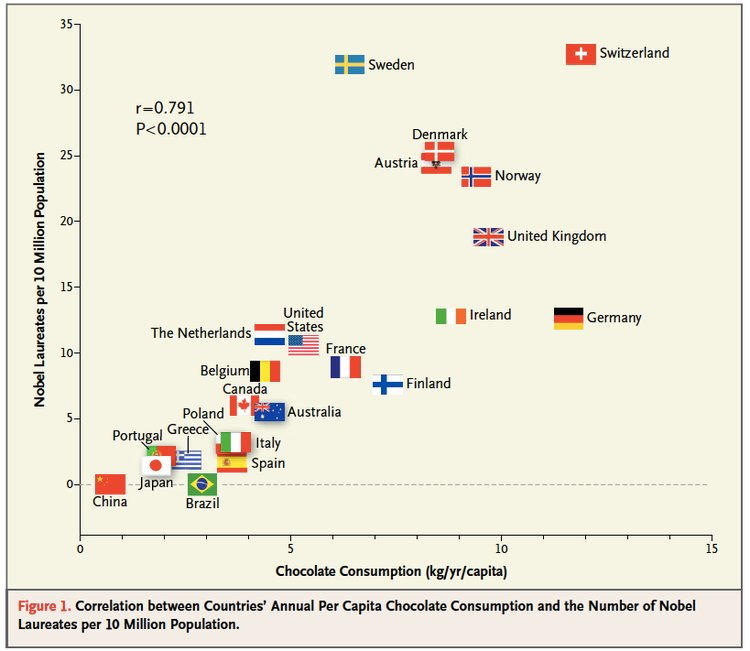
\includegraphics[width=0.9\textwidth]{Chocolate_Nobel.jpg}

\begin{frame}
\frametitle{Explanation}
\small
\begin{itemize}
\item Why isn't correlation enough?
\pause
\begin{itemize}
\item For \textbf{prediction}, correlation is fine: If we know a country has chocolate consumption of 10kg/yr/capita we can reasonably predict it will have about 25 Nobel Laureates
\pause
\item But for \textbf{intervention}, correlation does not help: forcing people to eat more chocolate does nothing on its own to produce more Nobel Laureates
\pause
\item For \textbf{explanation}, correlation also fails - it is no \textit{explanation} to say that Switzerland has the most Nobel Laureates because it has the highest chocolate consumption
\end{itemize}
\end{itemize}
\normalsize
\end{frame}

\begin{frame}
\frametitle{Explanation}
\begin{itemize}
\item Two perspectives on explanation:
\end{itemize}
\pause
\begin{table}[htbp]
  \centering
    \begin{tabular}{|>{\raggedright}p{5cm}|p{5cm}|}
    \toprule
    \textbf{Causes of Effects} & \textbf{Effects of Causes} \\
    \midrule
    What caused Y? & Does D cause Y? \\
    \midrule
    Why does Switzerland have so many Nobel laureates? & Does chocolate cause more Nobel laureates? \\
    \bottomrule
    \end{tabular}%
  \label{tab:addlabel}%
\end{table}%
\end{frame}

\begin{frame}
\frametitle{Explanation}
\begin{itemize}
\item Two perspectives on explanation:
\end{itemize}
\begin{multicols}{2}
\begin{knitrout}
\definecolor{shadecolor}{rgb}{0.969, 0.969, 0.969}\color{fgcolor}
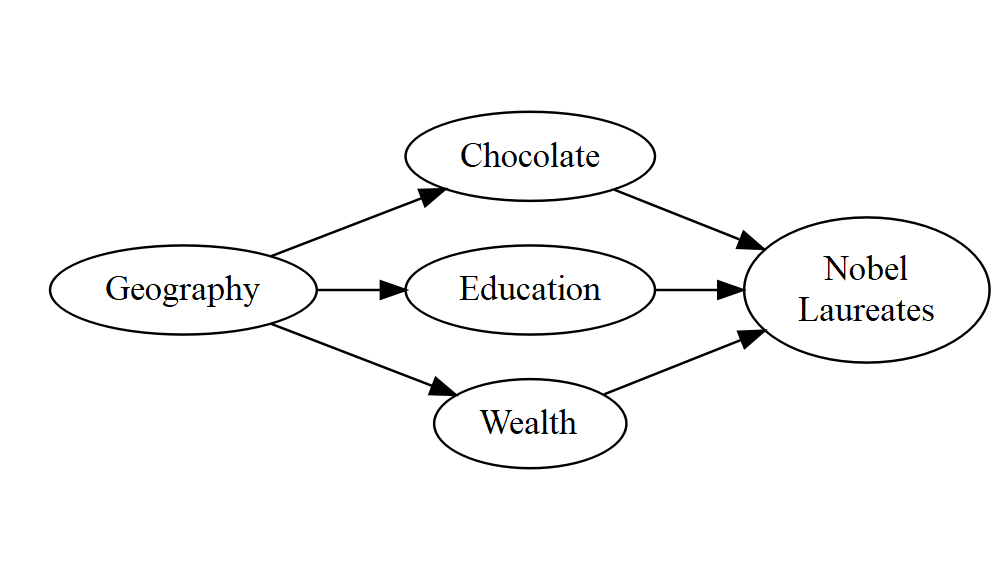
\includegraphics[width=\maxwidth]{figure/explanation1-1} 

\end{knitrout}
\pause
\begin{itemize}
\item Identifying the source of \textbf{ALL} of the variation in Nobel Laureates
\pause
\item An infinite task!
\end{itemize}
\pause
\columnbreak
\begin{knitrout}
\definecolor{shadecolor}{rgb}{0.969, 0.969, 0.969}\color{fgcolor}
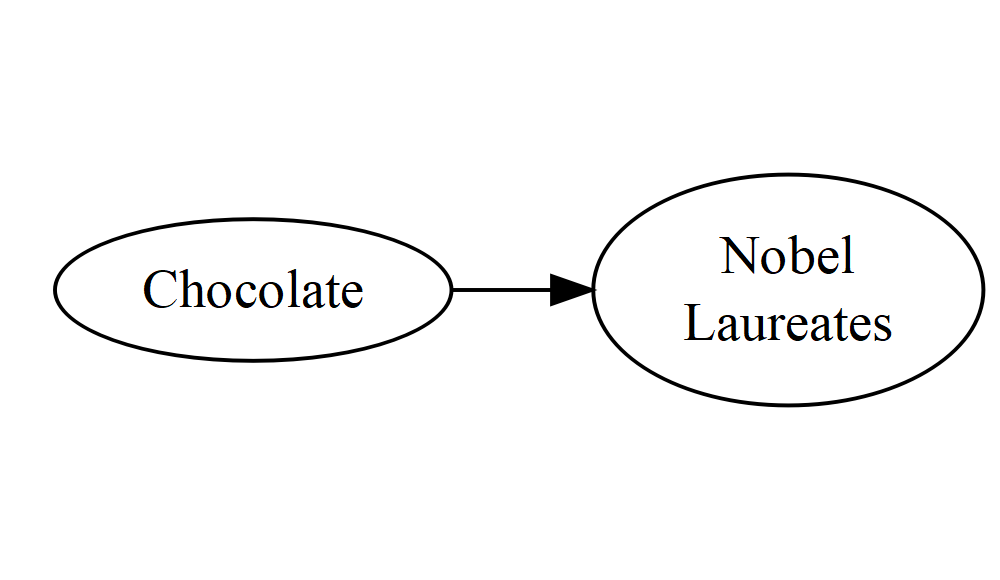
\includegraphics[width=\maxwidth]{figure/explanation2-1} 

\end{knitrout}
\pause
\begin{itemize}
\item Identifying how much \textbf{ONE} variable causes variation in Nobel Laureates
\pause
\item This we can do!
\end{itemize}
\end{multicols}
\end{frame}

\begin{frame}
\frametitle{Explanation}
\begin{itemize}
\item A focus on a single explanatory variable $D$ requires a clear definition of \textbf{'Treatment'}
\item AND to clearly define a \textbf{'Control'}
\begin{itemize}
\item What is the opposite of investing \$1bn in education?
\item No investment, or investing it elsewhere?
\end{itemize}
\item Define treatment:
\end{itemize}
\[D_i = 
\begin{cases}
1 \text{, if treated} \\
0 \text{, if not treated}
\end{cases}
\]
\end{frame}

\begin{frame}
\frametitle{Explanation}
\begin{itemize}
\item Defining our outcome:
\begin{itemize}
\item Is it the outcome we really care about? Or just what's easy to measure?
\item Tempting to look at many outcomes, but the risk of 'cherry-picking'
\begin{itemize}
\item All outcomes are \textbf{probabilistic} (due to all the other factors we haven't accounted for)
\item If we study 20 outcomes, on average one will show a significant effect even with no real causal effect
\end{itemize}
\item So we also want a \textbf{single outcome} usually
\end{itemize}
\end{itemize}
\end{frame}

\begin{frame}
\frametitle{Explanation}
\begin{itemize}
\item What are the \textbf{units} of our analysis?
\item Countries? Political Parties? Individuals?
\item eg. How does electoral system affect attitudes to redistribution?
\begin{itemize}
\item Treatment at the national level
\item Outcome at the individual level
\item Measurement needed at the lowest (individual) level
\end{itemize}
\item Units are \textbf{time-specific}: the same person 10 minutes later is a different unit
\end{itemize}
\end{frame}

\begin{frame}
\frametitle{Explanation}
\begin{multicols}{2}
Deterministic Explanation
\pause
\begin{itemize}
\item \textbf{Sufficient conditions:} Every time $D$ happens, $Y$ happens
\pause
\item \textbf{Necessary conditions:} $Y$ does not happen if $D$ does not happen ('\textit{but for}')
\end{itemize}
\pause
\columnbreak
Proababilistic Explanation
\pause
\begin{itemize}
\item If $D$ happens, the \textbf{probability} of $Y$ increases
\pause
\item Treatment effects are a distribution, not a single value
\end{itemize}
\end{multicols}
\end{frame}

\section{Causal Inference}

\begin{frame}
\frametitle{Causal Inference}
\begin{itemize}
\item The \textbf{causal effect} of treatment is how each unit's outcome differs when it is treated and not treated
\pause
\item This means comparing the \textbf{Potential Outcomes} for unit $i$:
\[
Y_{Di} = 
\begin{cases}
Y_{1i}\text{   Potential Outcome if unit i treated} \\
Y_{0i}\text{   Potential Outcome if unit i NOT treated}
\end{cases}
\]
\item Individual Treatment Effect for unit $i$: $\alpha_i = Y_{1i} - Y_{0i}$
\end{itemize}
\end{frame}

\begin{frame}
\frametitle{Causal Inference}
\begin{itemize}
\item The \textbf{causal effect} of treatment is how each unit's outcome differs when it is treated and not treated
\item This means comparing the \textbf{Potential Outcomes} for unit $i$:
\[
Y_{Di} = 
\begin{cases}
Y_{1i}\text{   GDP Growth of Brazil in 2010 if a Democracy} \\
Y_{0i}\text{   GDP Growth of Brazil in 2010 if NOT a Democracy}
\end{cases}
\]
\item Individual Treatment Effect for unit $i$: $\alpha_i = Y_{1i} - Y_{0i}$
\end{itemize}
\end{frame}

\begin{frame}
\frametitle{Causal Inference}
\begin{itemize}
\item We are relying on \textbf{counterfactuals}
\pause
\begin{itemize}
\item What would have happened to the same unit if the treatment had not happened?
\pause
\item Would World War I still have happened if Archduke Franz Ferdinand had not been assassinated in 1914?
\pause
\item Would Brazil have won the 2014 World Cup if Neymar had not been injured?
\pause
\end{itemize}
\end{itemize}
\end{frame}

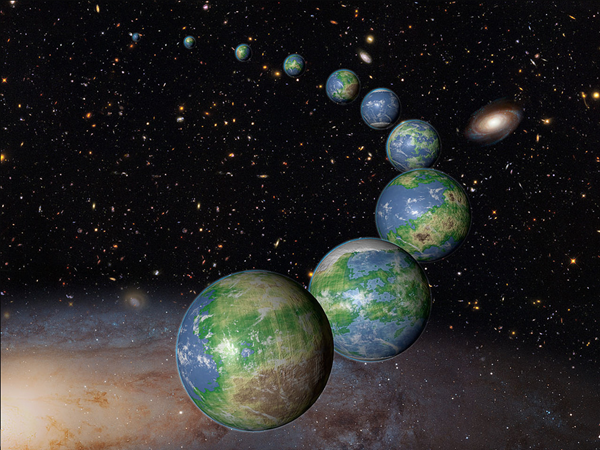
\includegraphics[width=1\textwidth]{figure/Multiverse.png}

\begin{frame}
\frametitle{Causal Inference}
\footnotesize
\begin{table}[htbp]
  \centering
  \caption{Potential Outcomes are just another Variable}
    \begin{tabular}{|p{2.4cm}|p{2.4cm}|p{2.4cm}|p{2.4cm}|}
    \hline
          & \multicolumn{1}{p{2.4cm}|}{GDP Growth if Democracy} & \multicolumn{1}{p{2.4cm}|}{GDP Growth if  NOT Democracy} &  Treatment Effect\bigstrut\\
    \hline
          & \multicolumn{1}{l|}{$Y_1$} & \multicolumn{1}{l|}{$Y_0$} & \multicolumn{1}{l|}{$Y_1-Y_0$} \bigstrut\\
    \hline
    Brasil & 4     & 1     & 3 \bigstrut\\
    \hline
    Argentina & 7    & 4     & 3 \bigstrut\\
    \hline
    Bolivia & 2     & 4     & -2 \bigstrut\\
    \hline
    Colombia & 7    & 7    & 0 \bigstrut\\
    \hline
    Peru & 5     & 4     & 1 \bigstrut\\
    \hline
    \end{tabular}%
  \label{tab:addlabel}%
\end{table}%
\normalsize
\end{frame}

\begin{frame}
\frametitle{Causal Inference}
\begin{itemize}
\item Political Science is not about explaining individual events
\pause
\item We ideally want general theories that apply to many situations
\pause
\item To explain a systematic treatment - not a single event - we need \textbf{multiple counterfactual comparisons}
\pause
\item We know how democracy works in Europe; the question is what will happen if it becomes more common in Africa?
\pause
\begin{block}{Average Treatment Effect}
\item We want to calculate an \textbf{Average Treatment Effect} 
\pause 
\item $$ATE=E(\alpha_i) = E (Y_1 - Y_0) = E(Y_1) - E(Y_0) = \frac{\sum_i (Y_{1i} - Y_{0i})}{N}$$
\end{block}
\end{itemize}
\end{frame}

\begin{frame}
\frametitle{Causal Inference}
\footnotesize
\begin{table}[htbp]
  \centering
  \caption{Potential Outcomes are just another Variable}
    \begin{tabular}{|p{2.4cm}|p{2.4cm}|p{2.4cm}|p{2.4cm}|}
    \hline
          & \multicolumn{1}{p{2.4cm}|}{GDP Growth if Democracy} & \multicolumn{1}{p{2.4cm}|}{GDP Growth if  NOT Democracy} & Treatment Effect \bigstrut\\
    \hline
          & \multicolumn{1}{p{2.4cm}|}{$Y_1$} & \multicolumn{1}{l|}{$Y_0$} & \multicolumn{1}{l|}{$Y_{1} - Y_{0}$} \bigstrut\\
    \hline
    Brasil & 4     & 1     & 3 \bigstrut\\
    \hline
    Argentina & 7    & 4     & 3 \bigstrut\\
    \hline
    Bolivia & 2     & 4     & -2 \bigstrut\\
    \hline
    Colombia & 7    & 7    & 0 \bigstrut\\
    \hline
    Peru & 5     & 4     & 1 \bigstrut\\
    \hline
    \textbf{Average Treatment Effect} & \textbf{5} & \textbf{4} & \textbf{1} \bigstrut\\
    \hline
    \end{tabular}%
  \label{tab:addlabel}%
\end{table}%
\normalsize
\end{frame}

\begin{frame}
\frametitle{Causal Inference}
\begin{block}{The Fundamental Problem of Causal Inference}
\begin{itemize}
\item No units can receive \textbf{both} treatment and control
\item So we can never observe both $Y_1$ and $Y_0$ for the same unit
\item \textit{Individual} Treatment Effects are \textbf{Impossible to Estimate}
\end{itemize}
\end{block}
\pause
\[
Y_{i}^{obs} = 
\begin{cases}
Y_{1i} \text{ if } D_i=1 \\
Y_{0i} \text{ if } D_i=0
\end{cases}
\]
\pause
$$Y_{i}^{obs} = D_i \cdot Y_{1i} + (1-D_i) \cdot Y_{0i}$$
\end{frame}

\begin{frame}
\frametitle{Causal Inference}
\footnotesize
\begin{table}[htbp]
  \centering
  \caption{Potential Outcomes Example}
    \begin{tabular}{|p{1.8cm}|p{1.8cm}|p{2cm}|p{2cm}|p{2cm}|}
    \hline
          & \multicolumn{1}{p{1.8cm}|}{Democracy?} & \multicolumn{1}{p{2cm}|}{GDP Growth if Democracy} & \multicolumn{1}{p{2.2cm}|}{GDP Growth if NOT Democracy} &  Treatment Effect \bigstrut\\
    \hline
          & \multicolumn{1}{p{1.8cm}|}{$D_i$} & \multicolumn{1}{p{2cm}|}{$Y_1$} & \multicolumn{1}{p{2.2cm}|}{$Y_0$} & \multicolumn{1}{p{1.8cm}|}{$Y_{1} - Y_{0}$} \bigstrut\\
    \hline
    Brasil & 1 & 4     & 1      & 3 \bigstrut\\
    \hline
    Argentina & 0 & 7    & 4      & 3 \bigstrut\\
    \hline
    Bolivia & 1 & 2     & 4     & -2 \bigstrut\\
    \hline
    Colombia & 0 &  7   & 7    & 0 \bigstrut\\
    \hline
    Peru & 0 & 5     & 4     & 1 \bigstrut\\
\hline
    \end{tabular}%
  \label{tab:addlabel}%
\end{table}%
\normalsize
\end{frame}

\begin{frame}
\frametitle{Causal Inference}
\footnotesize
\begin{table}[htbp]
  \centering
  \caption{Potential Outcomes Example}
    \begin{tabular}{|p{1.8cm}|p{1.8cm}|p{2cm}|p{2cm}|p{2cm}|}
    \hline
          & \multicolumn{1}{p{1.8cm}|}{Democracy?} & \multicolumn{1}{p{2cm}|}{GDP Growth if Democracy} & \multicolumn{1}{p{2.2cm}|}{GDP Growth if NOT Democracy} & Treatment Effect \bigstrut\\
    \hline
          & \multicolumn{1}{p{1.8cm}|}{$D_i$} & \multicolumn{1}{p{2cm}|}{$Y_1$} & \multicolumn{1}{p{2.2cm}|}{$Y_0$} & \multicolumn{1}{p{1.8cm}|}{$Y_{1} - Y_{0}$} \bigstrut\\
    \hline
    Brasil & 1 & 4     & ?      & ? \bigstrut\\
    \hline
    Argentina & 0 & ?    & 4      & ? \bigstrut\\
    \hline
    Bolivia & 1 & 2     & ?     & ? \bigstrut\\
    \hline
    Colombia & 0 &  ?   & 7    & ? \bigstrut\\
    \hline
    Peru & 0 & ?     & 4     & ? \bigstrut\\
\hline
    \end{tabular}%
  \label{tab:addlabel}%
\end{table}%
\normalsize
\end{frame}

\begin{frame}
\frametitle{Causal Inference}
\footnotesize
\begin{table}[htbp]
  \centering
  \caption{Potential Outcomes Example}
    \begin{tabular}{|p{1.8cm}|p{1.8cm}|p{2cm}|p{2cm}|p{2cm}|}
    \hline
          & \multicolumn{1}{p{1.8cm}|}{Democracy?} & \multicolumn{1}{p{2cm}|}{GDP Growth if Democracy} & \multicolumn{1}{p{2.2cm}|}{GDP Growth if NOT Democracy} & \textbf{Observed} GDP Growth \bigstrut\\
    \hline
          & \multicolumn{1}{p{1.8cm}|}{$D_i$} & \multicolumn{1}{p{2cm}|}{$Y_1$} & \multicolumn{1}{p{2.2cm}|}{$Y_0$} & \multicolumn{1}{p{1.8cm}|}{$Y^{obs}$} \bigstrut\\
    \hline
    Brasil & 1 & 4     & ?      & 4 \bigstrut\\
    \hline
    Argentina & 0 & ?    & 4      & 4 \bigstrut\\
    \hline
    Bolivia & 1 & 2     & ?     & 2 \bigstrut\\
    \hline
    Colombia & 0 &  ?   & 7    & 7 \bigstrut\\
    \hline
    Peru & 0 & ?     & 4     & 4 \bigstrut\\
    \hline
    \end{tabular}%
  \label{tab:addlabel}%
\end{table}%
\normalsize
\end{frame}

\begin{frame}
\frametitle{Causal Inference}
\begin{itemize}
\item Actually, nothing stops us calculating the \textbf{Average Treatment Effect}
\pause
\item The question is, is the ATE accurate? \pause No!
\pause
\end{itemize}
\footnotesize
\begin{table}[htbp]
  \centering
    \begin{tabular}{|p{1.8cm}|p{1.8cm}|p{2cm}|p{2cm}|p{2cm}|}
    \hline
          & \multicolumn{1}{p{1.8cm}|}{Democracy?} & \multicolumn{1}{p{2cm}|}{GDP Growth if Democracy} & \multicolumn{1}{p{2.2cm}|}{GDP Growth if NOT Democracy} & \textbf{Treatment Effect} \bigstrut\\
    \hline
          & \multicolumn{1}{p{1.8cm}|}{$D_i$} & \multicolumn{1}{p{2cm}|}{$Y_1$} & \multicolumn{1}{p{2.2cm}|}{$Y_0$} & \multicolumn{1}{p{1.8cm}|}{$Y_{1} - Y_{0}$} \bigstrut\\
    \hline
    Brasil & 1 & 4     & ?      & ? \bigstrut\\
    \hline
    Argentina & 0 & ?    & 4      & ? \bigstrut\\
    \hline
    Bolivia & 1 & 2     & ?     & ? \bigstrut\\
    \hline
    Colombia & 0 &  ?   & 7    & ? \bigstrut\\
    \hline
    Peru & 0 & ?     & 4     & ? \bigstrut\\
    \hline
    \textbf{Average Treatment Effect} & & \textbf{3} & \textbf{5} & \textbf{-2} \bigstrut\\
    \hline
    \end{tabular}%
  \label{tab:addlabel}%
\end{table}%
\normalsize
\end{frame}

\begin{frame}
\frametitle{Causal Inference}
\begin{itemize}
\item \textbf{So what went wrong?}
\pause
\item The potential outcomes we \textbf{observe} are a \textbf{biased representation} of the potential outcomes of all the units
\pause
\end{itemize}
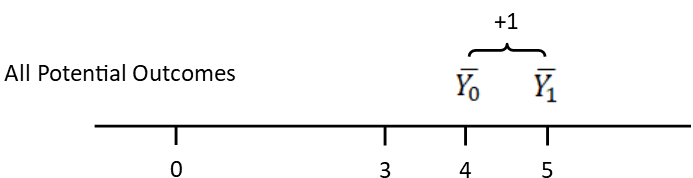
\includegraphics[width=0.9\textwidth]{PO_number_line_1.png}
\end{frame}

\begin{frame}
\frametitle{Causal Inference}
\begin{itemize}
\item \textbf{So what went wrong?}
\item The potential outcomes we \textbf{observe} are a \textbf{biased representation} of the potential outcomes of all the units
\end{itemize}
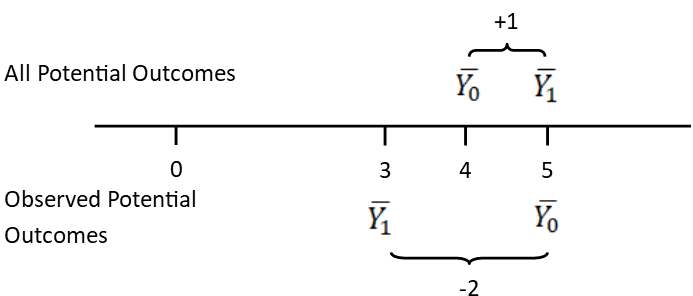
\includegraphics[width=0.9\textwidth]{PO_number_line_2.png}
\begin{itemize}
\item $E(Y_1)$ values are \textbf{biased lower} in the observed data
\pause
\item $E(Y_0)$ values are \textbf{biased higher} in the observed data
\pause
\item So $E(Y_1)-E(Y_0)$ is \textbf{biased}
\end{itemize}
\end{frame}

\begin{frame}
\frametitle{Causal Inference}
\begin{knitrout}
\definecolor{shadecolor}{rgb}{0.969, 0.969, 0.969}\color{fgcolor}
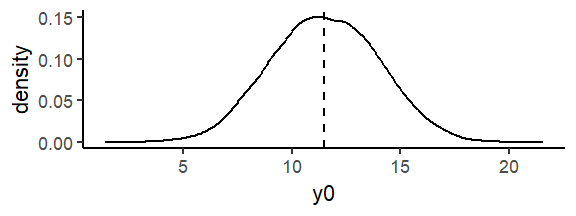
\includegraphics[width=\maxwidth]{figure/OVB1a-1} 

\end{knitrout}
\pause
\begin{knitrout}
\definecolor{shadecolor}{rgb}{0.969, 0.969, 0.969}\color{fgcolor}
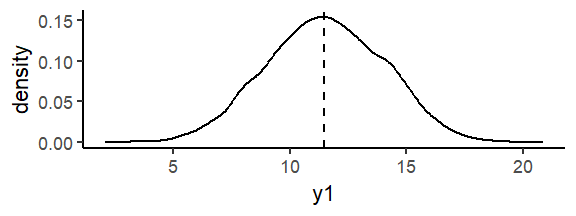
\includegraphics[width=\maxwidth]{figure/OVB2a-1} 

\end{knitrout}
\end{frame}

\begin{frame}
\frametitle{Causal Inference}
\begin{knitrout}
\definecolor{shadecolor}{rgb}{0.969, 0.969, 0.969}\color{fgcolor}
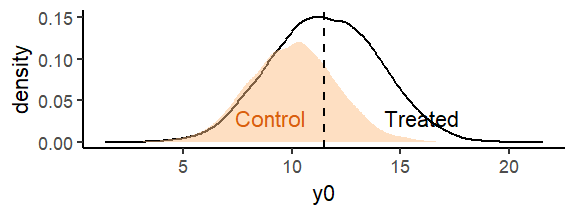
\includegraphics[width=\maxwidth]{figure/OVB1b-1} 

\end{knitrout}

\begin{knitrout}
\definecolor{shadecolor}{rgb}{0.969, 0.969, 0.969}\color{fgcolor}
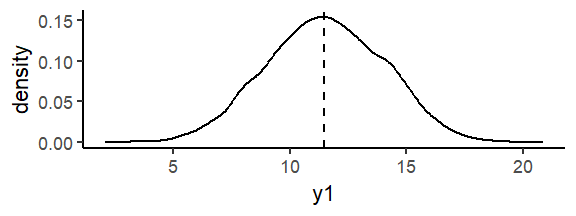
\includegraphics[width=\maxwidth]{figure/OVB2b-1} 

\end{knitrout}
\end{frame}

\begin{frame}
\frametitle{Causal Inference}
\begin{knitrout}
\definecolor{shadecolor}{rgb}{0.969, 0.969, 0.969}\color{fgcolor}
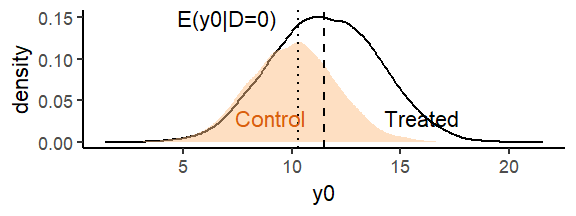
\includegraphics[width=\maxwidth]{figure/OVB1c-1} 

\end{knitrout}

\begin{knitrout}
\definecolor{shadecolor}{rgb}{0.969, 0.969, 0.969}\color{fgcolor}
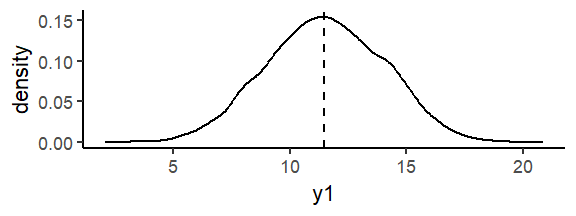
\includegraphics[width=\maxwidth]{figure/OVB2c-1} 

\end{knitrout}
\end{frame}

\begin{frame}
\frametitle{Causal Inference}
\begin{knitrout}
\definecolor{shadecolor}{rgb}{0.969, 0.969, 0.969}\color{fgcolor}
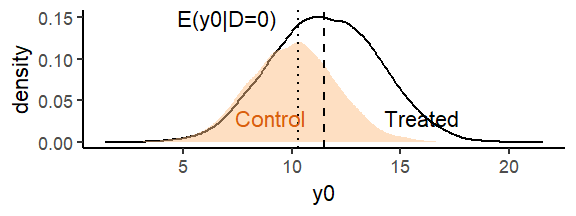
\includegraphics[width=\maxwidth]{figure/OVB1d-1} 

\end{knitrout}

\begin{knitrout}
\definecolor{shadecolor}{rgb}{0.969, 0.969, 0.969}\color{fgcolor}
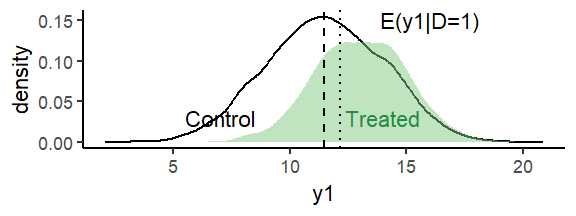
\includegraphics[width=\maxwidth]{figure/OVB2d-1} 

\end{knitrout}
\end{frame}

\begin{frame}
\frametitle{Causal Inference}
\begin{itemize}
\item Contrasting the averages of the hypothetical variables and the observed variables:
\end{itemize}
\begin{table}[htbp]
  \centering
    \begin{tabular}{|c|l|l|l|}
    \hline
          &       & \multicolumn{2}{c|}{Hypothetical outcome} \bigstrut\\
    \hline
          &       & $Y0$    & $Y1$ \bigstrut\\
    \hline
    \multirow{2}[4]{*}{Actual Treatment} & $D=0$   & $E(Y_{0i}|D=0)$ & $E(Y_{1i}|D=0)$ \bigstrut\\
\cline{2-4}          & $D=1$   & $E(Y_{0i}|D=1)$ & $E(Y_{1i}|D=1)$ \bigstrut\\
    \hline
    \end{tabular}%
  \label{tab:addlabel}%
\end{table}%

\end{frame}

\begin{frame}
\frametitle{Causal Inference}
\begin{itemize}
\item All our causal estimates are \textbf{averages}
\begin{itemize}
\item We cannot distinguish the null hypothesis of no average effect from the sharp null hypothesis of no individual effects
\end{itemize}
\footnotesize
\begin{table}[htbp]
  \centering
    \begin{tabular}{|l|p{3cm}|p{3cm}|}
    \hline
          & \multicolumn{1}{p{3cm}|}{No Average Effect ($Y_1-Y_0$)} & \multicolumn{1}{p{3cm}|}{"Sharp null": No individual effects ($Y_1-Y_0$)} \bigstrut\\
    \hline
    Brasil & 2     & 0 \bigstrut\\
    \hline
    Argentina & -1    & 0 \bigstrut\\
    \hline
    Bolivia & 1     & 0 \bigstrut\\
    \hline
    Colombia & 0     & 0 \bigstrut\\
    \hline
    Peru  & -2    & 0 \bigstrut\\
    \hline
    \textbf{Average} & \textbf{0}     & \textbf{0} \bigstrut\\
    \hline
    \end{tabular}%
  \label{tab:addlabel}%
\end{table}%
\normalsize
\end{itemize}
\end{frame}

\section{Why Observational Data is Biased}

\begin{frame}
\frametitle{Bias}
\begin{itemize}
\item Why are potential outcomes biased in our data?
\begin{enumerate}
\item Omitted Variables
\item Reverse Causation
\item Selection Bias
\end{enumerate}
\item \textbf{In all of these cases the potential outcomes are distorted so basic regression is biased}
\end{itemize}
\end{frame}

\begin{frame}
\frametitle{Omitted Variable Bias}
\begin{multicols}{2}
A real causal relationship:
\begin{knitrout}
\definecolor{shadecolor}{rgb}{0.969, 0.969, 0.969}\color{fgcolor}
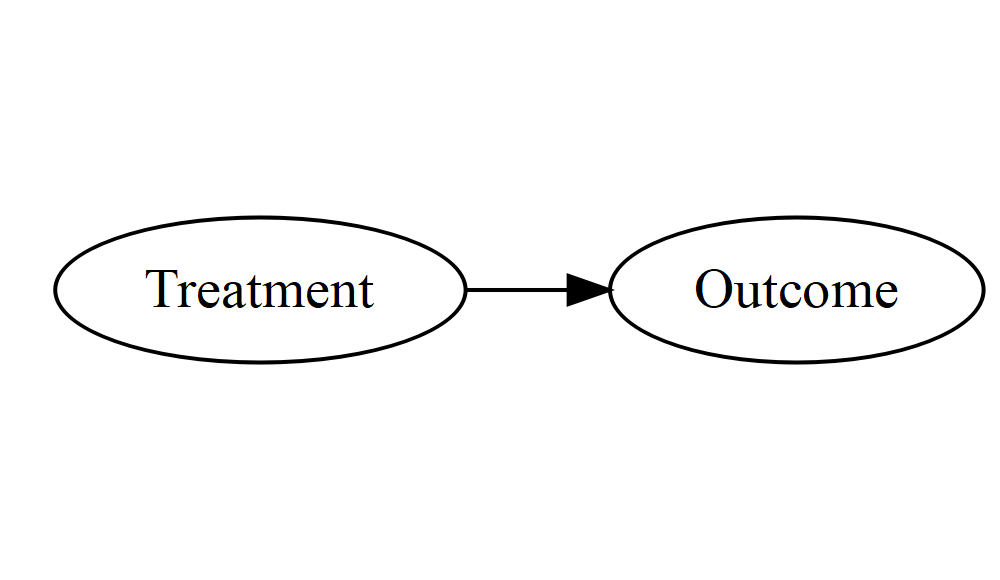
\includegraphics[width=\maxwidth]{figure/explanation3-1} 

\end{knitrout}
\columnbreak
Being misled by omitted variable bias:
\begin{knitrout}
\definecolor{shadecolor}{rgb}{0.969, 0.969, 0.969}\color{fgcolor}
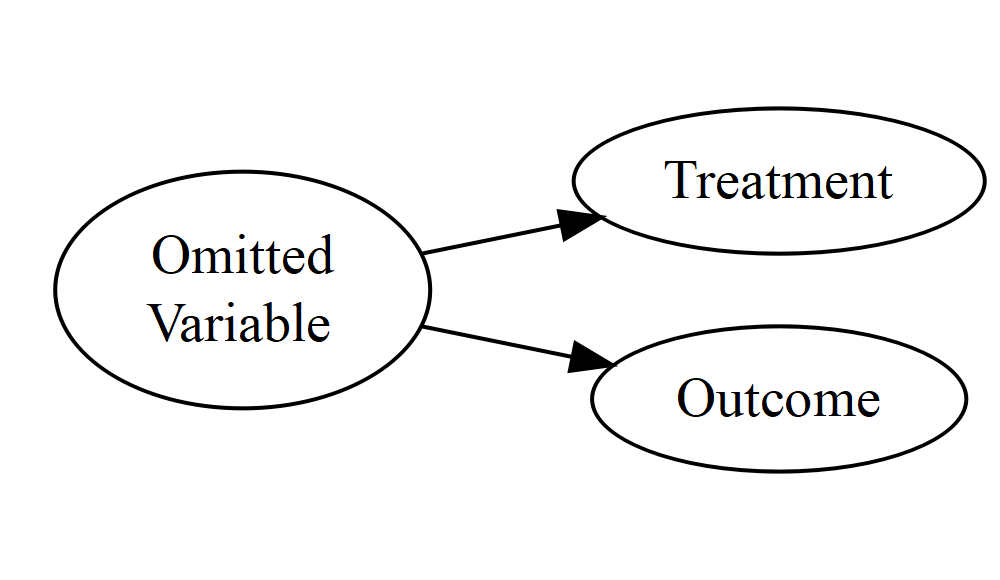
\includegraphics[width=\maxwidth]{figure/explanation4-1} 

\end{knitrout}
\end{multicols}
\begin{itemize}
\pause
\item A third variable causes some units to have \textbf{different values of potential outcomes}, AND for those \textbf{same units to be treated}
\pause
\item So treated units have non-representative $Y_1$
\item And control units have non-representative $Y_0$
\end{itemize}
\end{frame}

\begin{frame}
\frametitle{Omitted Variable Bias}
\begin{multicols}{2}
A real causal relationship:
\begin{knitrout}
\definecolor{shadecolor}{rgb}{0.969, 0.969, 0.969}\color{fgcolor}
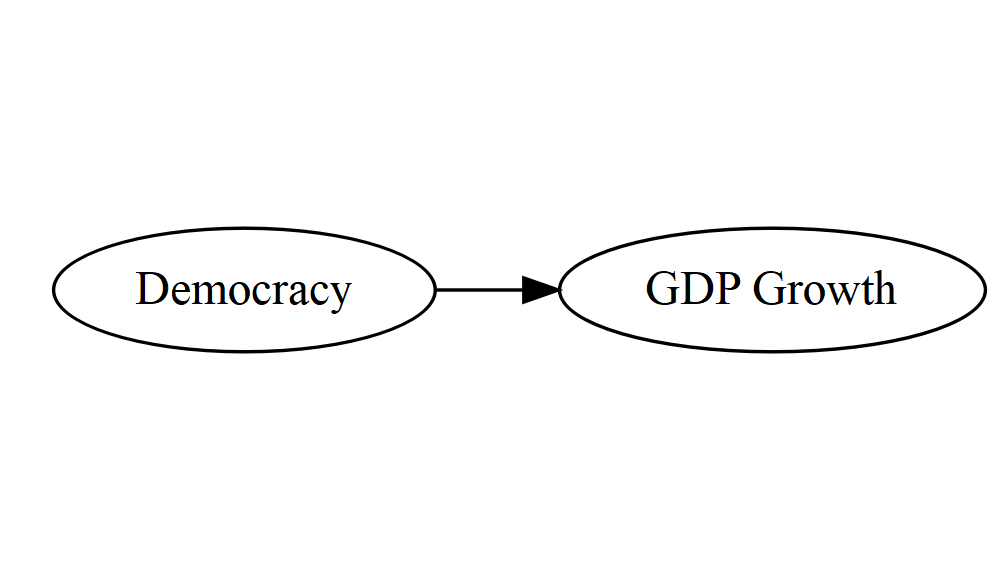
\includegraphics[width=\maxwidth]{figure/explanation9-1} 

\end{knitrout}
\columnbreak
Being misled by omitted variable bias:
\begin{knitrout}
\definecolor{shadecolor}{rgb}{0.969, 0.969, 0.969}\color{fgcolor}
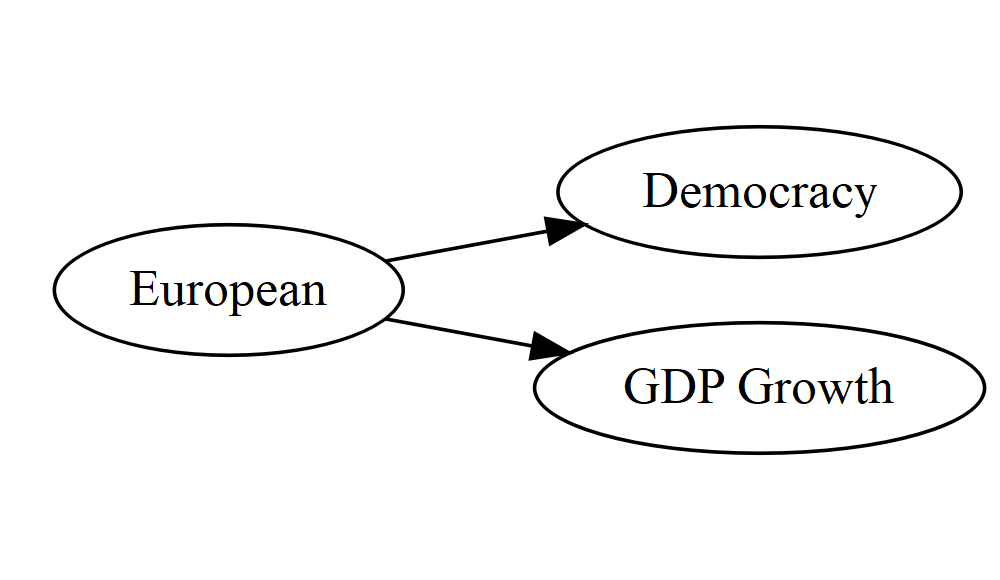
\includegraphics[width=\maxwidth]{figure/explanation10-1} 

\end{knitrout}
\end{multicols}
\begin{itemize}
\pause
\item European countries faced conditions that encouraged both democracy and rapid GDP growth
\end{itemize}
\end{frame}

\begin{frame}
\frametitle{Omitted Variable Bias}
\begin{knitrout}
\definecolor{shadecolor}{rgb}{0.969, 0.969, 0.969}\color{fgcolor}
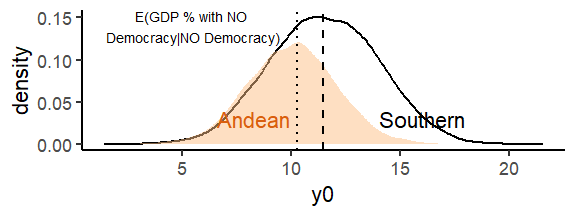
\includegraphics[width=\maxwidth]{figure/OVB3-1} 

\end{knitrout}

\begin{knitrout}
\definecolor{shadecolor}{rgb}{0.969, 0.969, 0.969}\color{fgcolor}
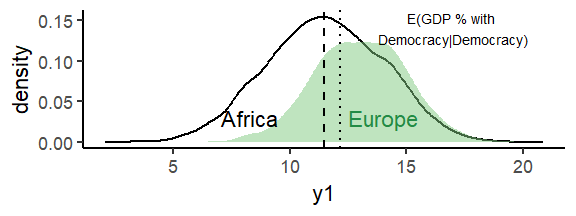
\includegraphics[width=\maxwidth]{figure/OVB4-1} 

\end{knitrout}
\end{frame}

\begin{frame}
\frametitle{Omitted Variable Bias}
\begin{itemize}
\item Let's say that $Y_{1i} = Y_{0i} + \alpha$, where $\alpha$ is the real constant treatment effect
\end{itemize}
$$ \hat{ATE} = E(Y_1|D=1) - E(Y_0|D=0)$$ \\ \pause
$$ \hat{ATE} = \alpha + E(Y_0|D=1) - E(Y_0|D=0)$$ \\ \pause
$$ \hat{ATE} = \text{Real ATE} + \text{Bias}   \\
\end{frame}


\begin{frame}
\frametitle{Reverse Causation}
\begin{multicols}{2}
A real causal relationship:
\begin{knitrout}
\definecolor{shadecolor}{rgb}{0.969, 0.969, 0.969}\color{fgcolor}
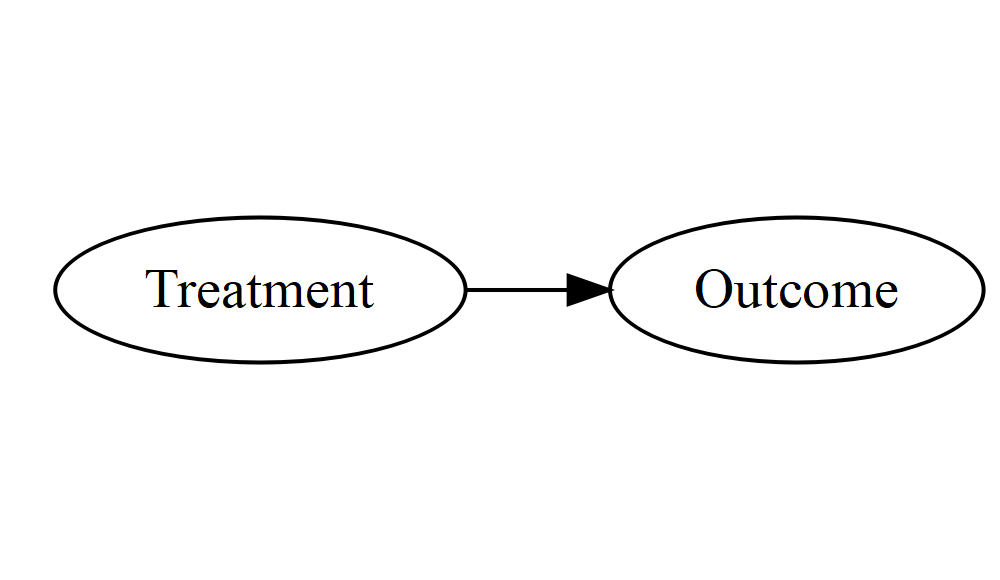
\includegraphics[width=\maxwidth]{figure/explanation5-1} 

\end{knitrout}
\columnbreak
Being misled by reverse causation:
\begin{knitrout}
\definecolor{shadecolor}{rgb}{0.969, 0.969, 0.969}\color{fgcolor}
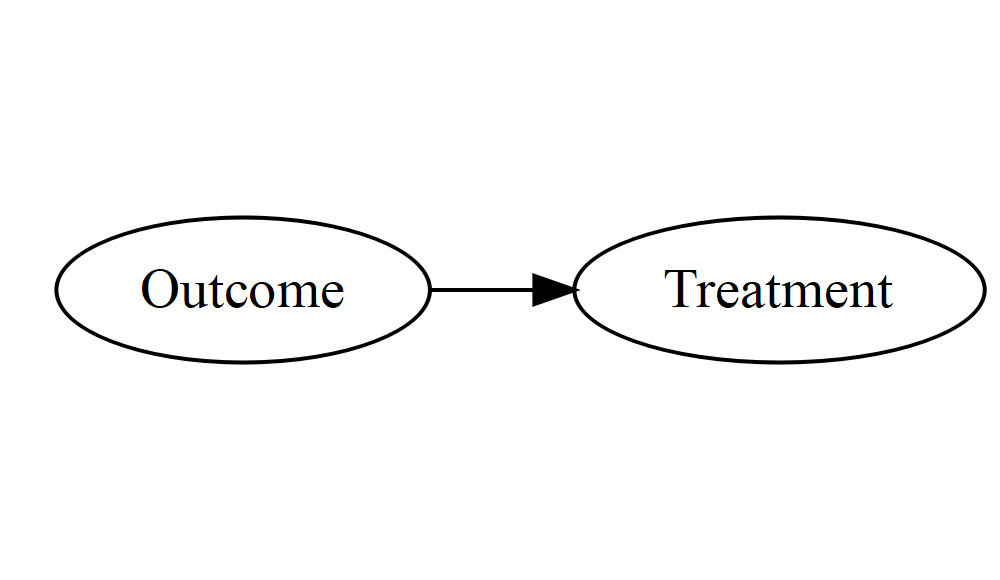
\includegraphics[width=\maxwidth]{figure/explanation6-1} 

\end{knitrout}
\end{multicols}
\begin{itemize}
\pause
\item $D$ does not affect $Y$, but higher $Y$ makes treatment ($D$) more likely
\pause
\item So the two variables are correlated
\end{itemize}
\end{frame}

\begin{frame}
\frametitle{Reverse Causation}
\begin{multicols}{2}
A real causal relationship:
\begin{knitrout}
\definecolor{shadecolor}{rgb}{0.969, 0.969, 0.969}\color{fgcolor}
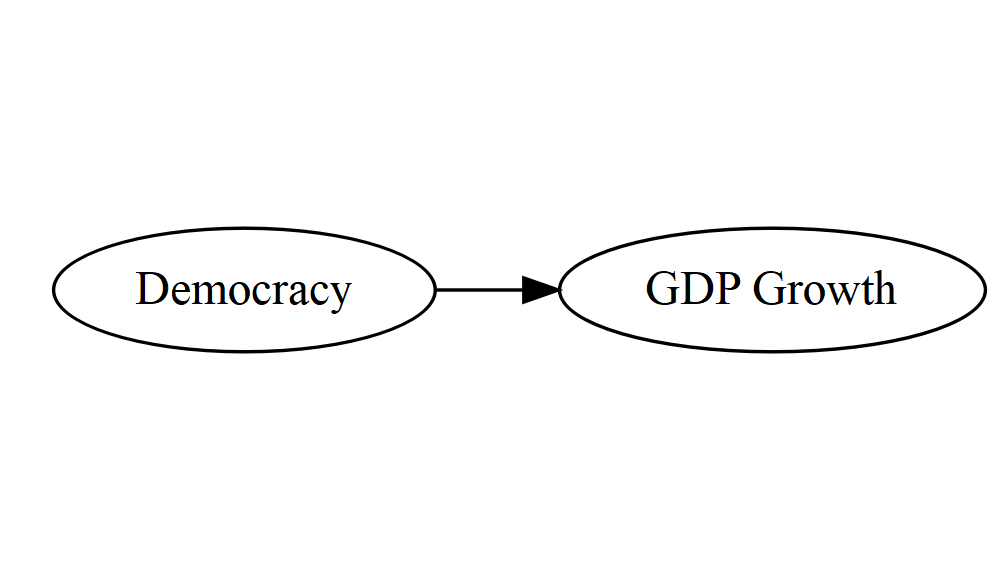
\includegraphics[width=\maxwidth]{figure/reverse1-1} 

\end{knitrout}
\columnbreak
Being misled by reverse causation:
\begin{knitrout}
\definecolor{shadecolor}{rgb}{0.969, 0.969, 0.969}\color{fgcolor}
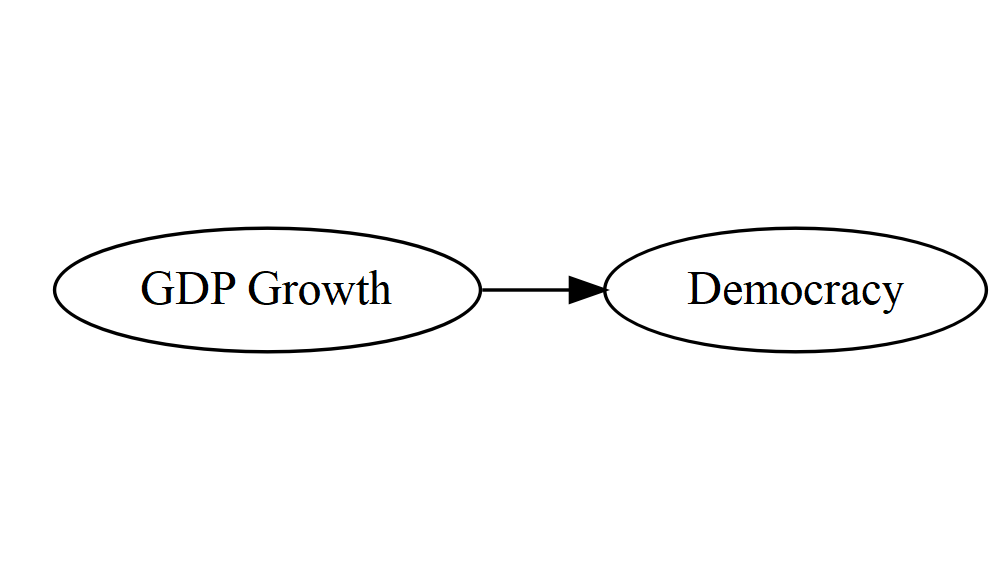
\includegraphics[width=\maxwidth]{figure/reverse2-1} 

\end{knitrout}
\end{multicols}
\begin{itemize}
\pause
\item GDP Growth encourages democratization
\pause
\item So democracies are more likely to have experienced high growth rates
\end{itemize}
\end{frame}

\begin{frame}
\frametitle{Reverse Causation}
\begin{knitrout}
\definecolor{shadecolor}{rgb}{0.969, 0.969, 0.969}\color{fgcolor}
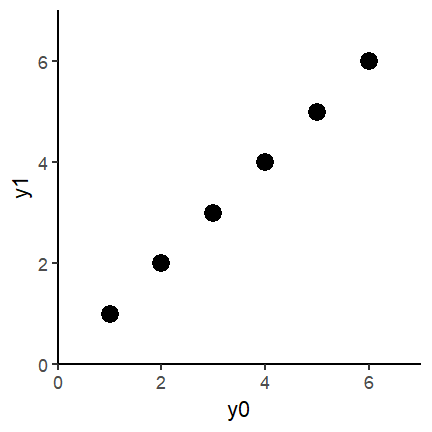
\includegraphics[width=\maxwidth]{figure/reverse3-1} 

\end{knitrout}
\begin{itemize}
\item $E(Y_1-Y_0) = 0$
\end{itemize}
\end{frame}

\begin{frame}
\frametitle{Reverse Causation}
\begin{knitrout}
\definecolor{shadecolor}{rgb}{0.969, 0.969, 0.969}\color{fgcolor}
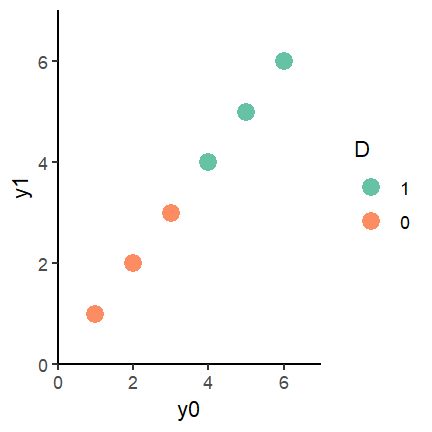
\includegraphics[width=\maxwidth]{figure/reverse5-1} 

\end{knitrout}
\end{frame}

\begin{frame}
\frametitle{Reverse Causation}
\begin{knitrout}
\definecolor{shadecolor}{rgb}{0.969, 0.969, 0.969}\color{fgcolor}
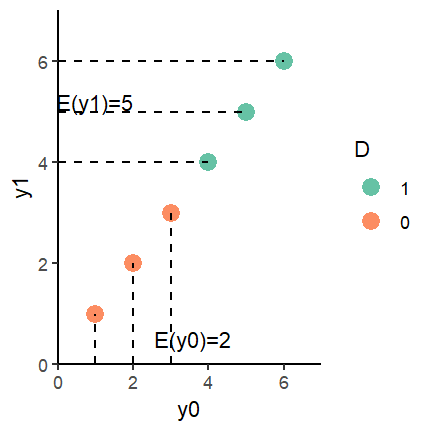
\includegraphics[width=\maxwidth]{figure/reverse6-1} 

\end{knitrout}
\begin{itemize}
\pause
\item $E(Y_1|D=1)-E(Y_0|D=0) = 5 - 2 = 3$
\end{itemize}
\end{frame}

\begin{frame}
\frametitle{Selection Bias}
\begin{multicols}{2}
A real causal relationship:
\begin{knitrout}
\definecolor{shadecolor}{rgb}{0.969, 0.969, 0.969}\color{fgcolor}
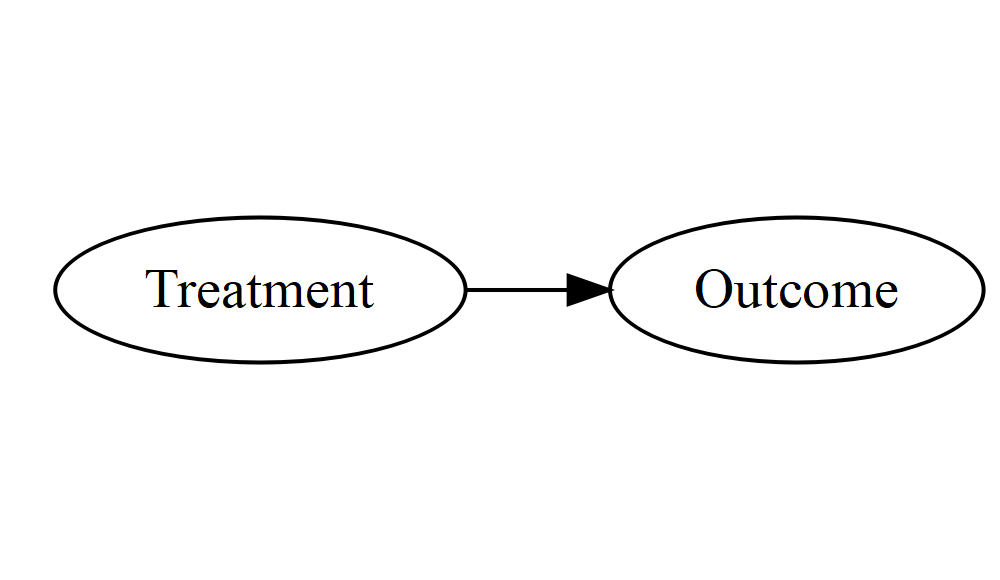
\includegraphics[width=\maxwidth]{figure/explanation7-1} 

\end{knitrout}
\columnbreak
Being misled by Selection Bias:
\begin{knitrout}
\definecolor{shadecolor}{rgb}{0.969, 0.969, 0.969}\color{fgcolor}
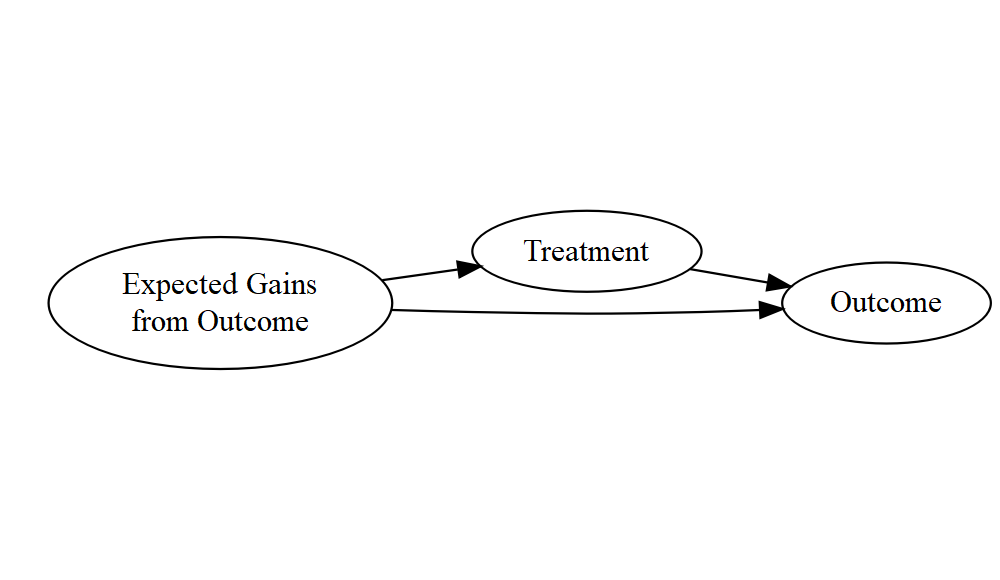
\includegraphics[width=\maxwidth]{figure/explanation8-1} 

\end{knitrout}
\end{multicols}
\end{frame}

\begin{frame}
\frametitle{Selection Bias}
\begin{multicols}{2}
A real causal relationship:
\begin{knitrout}
\definecolor{shadecolor}{rgb}{0.969, 0.969, 0.969}\color{fgcolor}
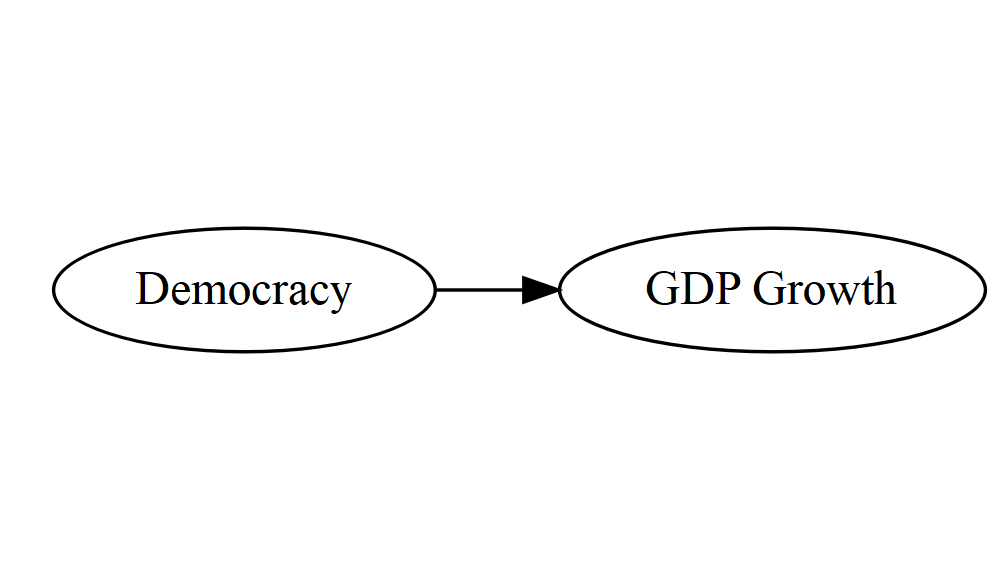
\includegraphics[width=\maxwidth]{figure/explanation9b-1} 

\end{knitrout}
\columnbreak
Being misled by Selection Bias:
\begin{knitrout}
\definecolor{shadecolor}{rgb}{0.969, 0.969, 0.969}\color{fgcolor}
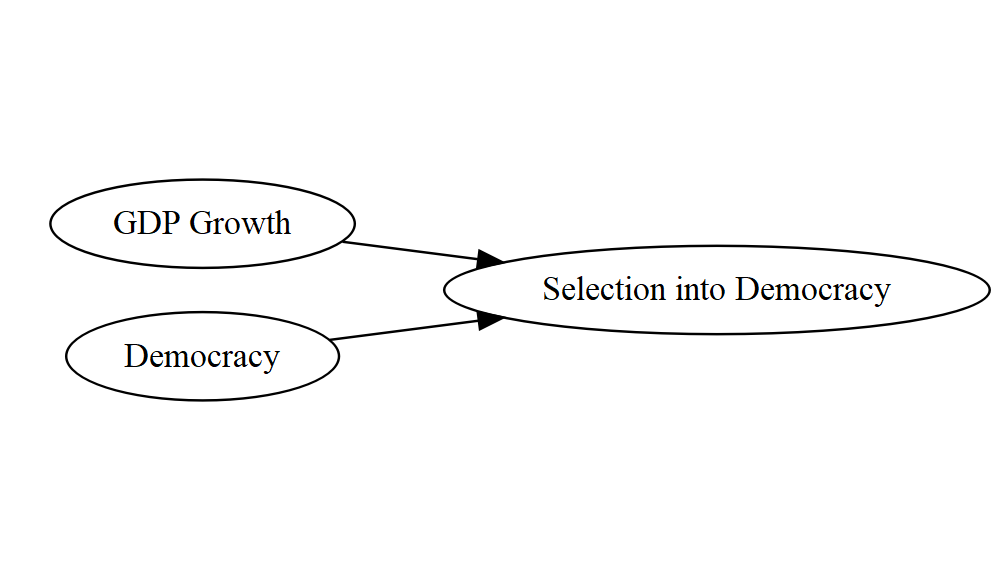
\includegraphics[width=\maxwidth]{figure/explanation10b-1} 

\end{knitrout}
\end{multicols}
\begin{itemize}
\pause
\item The units which benefit most from treatment (largest $y_1-y_0$) \textbf{choose treatment}
\pause
\item We don't see any of the low $y_1$'s of units which avoid treatment
\end{itemize}
\end{frame}

\begin{frame}
\frametitle{Self-Selection Bias}
\begin{knitrout}
\definecolor{shadecolor}{rgb}{0.969, 0.969, 0.969}\color{fgcolor}
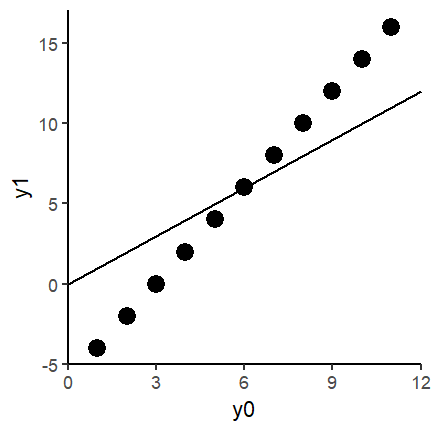
\includegraphics[width=\maxwidth]{figure/SSB1-1} 

\end{knitrout}
\begin{itemize}
\pause
\item Countries which can boost their GDP growth by becoming a democracy choose to democratize
\pause
\item Ex. Mexico? Myanmar?
\end{itemize}
\end{frame}

\begin{frame}
\frametitle{Self-Selection Bias}
\begin{knitrout}
\definecolor{shadecolor}{rgb}{0.969, 0.969, 0.969}\color{fgcolor}
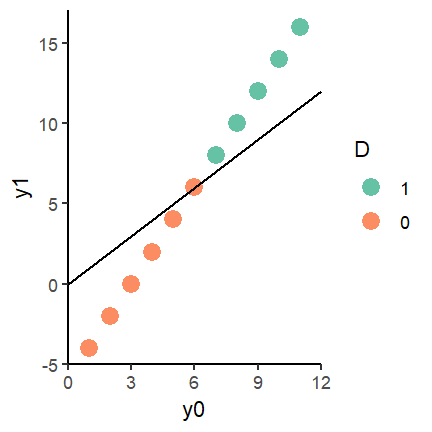
\includegraphics[width=\maxwidth]{figure/SSB2-1} 

\end{knitrout}
\begin{itemize}
\item $E(y_1)-E(y_0)=0$
\end{itemize}
\end{frame}

\begin{frame}
\frametitle{Self-Selection Bias}
\begin{knitrout}
\definecolor{shadecolor}{rgb}{0.969, 0.969, 0.969}\color{fgcolor}
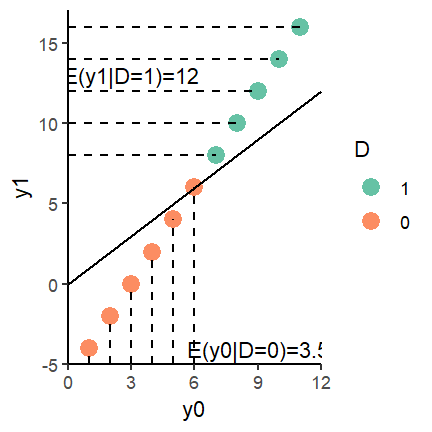
\includegraphics[width=\maxwidth]{figure/SSB3-1} 

\end{knitrout}
\begin{itemize}
\item $E(y_1|D=1)-E(y_0|D=0)=8.5$
\end{itemize}
\end{frame}

\begin{frame}
\frametitle{Self-Selection Bias}
\begin{itemize}
\item Allow treatment effects to vary across individuals, so $Y_{1i} = Y_{0i} + \alpha_i$
\end{itemize}
\begin{multline}
\underbrace{E(Y_i|D=1)-E(Y_i|D=0)}_\text{Observed Effect} = \underbrace{E(Y_{1i} - Y_{0i})}_\text{Real ATE} \\ + \underbrace{\frac{1}{2}\Big[ E(Y_{1i}|D=1) - E(Y_{1i}|D=0) \Big]}_\text{Imbalance on $Y_1$} + \underbrace{\frac{1}{2}\Big[ E(Y_{0i}|D=1) - E(Y_{0i}|D=0) \Big]}_\text{Imbalance on $Y_0$}
\end{multline}
\footnotesize
NB: For equal-sized treatment and control groups
\normalsize\end{frame}

\begin{frame}
\frametitle{Causal Inference}
\begin{itemize}
\item In all of these cases, \textbf{which units receive 'treatment' ($D_i=1$)}, and why, affect our estimate of the relationship between $D$ and $Y$
\pause
\begin{itemize}
\item This is the \textbf{Treatment Assignment Mechanism}
\pause
\end{itemize}
\item Messy treatment assignment mechanisms are why basic regression is no use for explanation
\pause
\begin{itemize}
\item It means our comparison control cases are really misleading
\pause
\item $Y_0$ for Malaysia is not a good guide to the $Y_0$ for Switzerland
\pause
\item What would happen if the 'untreated' units got treated?
\end{itemize}
\end{itemize}
\end{frame}


\begin{frame}
\frametitle{Causal Inference}
\begin{itemize}
\item The comparability of treatment and control units depends on how they got to be treated
\pause
\begin{block}{Treatment Assignment Mechanism}
\item The set of factors that determine why some units have $D=0$ and others have $D=1$
\end{block}
\end{itemize}
\end{frame}

\begin{frame}
\frametitle{Causal Inference}
\begin{itemize}
\item Explanation is more reliable where the \textbf{Treatment Assignment Mechanism is Independent of Potential Outcomes}
\pause
\begin{itemize}
\item Independent means the values of the potential outcomes give us no information about whether that unit was treated
\pause
\item $(Y_1,Y_0) \perp D$
\pause
\item $Pr(D|(Y_1,Y_0)) = Pr(D)$
\pause
\item $E(Y|D=1) = E(Y|D=0)$
\item Potential outcomes are 'balanced' across control and treatment groups
\end{itemize}
\end{itemize}
\end{frame}

\section{Rest of the Course}

\begin{frame}
\frametitle{Causal Inference}
\begin{itemize}
\item The rest of the course is mostly about the types of treatment assignment mechanisms that \textbf{avoid these biases} and provide plausible counterfactuals
\end{itemize}
\end{frame}

\begin{frame}
\frametitle{Causal Inference}
\begin{enumerate}
\item \textbf{Controlled Experiments} where we \textbf{control} the treatment assignment
\begin{itemize}
\item Field Experiments
\item Survey Experiments
\item Lab Experiments
\end{itemize}
\end{enumerate}
\end{frame}

\begin{frame}
\frametitle{Causal Inference}
\begin{enumerate}
 \setcounter{enumi}{1}
\item \textbf{Natural Experiments} where the assignment mechanism creates balanced potential outcomes
\begin{itemize}
\item Randomized natural experiments
\item Regression Discontinuities
\item Instrumental Variables
\end{itemize}
\end{enumerate}
\end{frame}

\begin{frame}
\frametitle{Causal Inference}
\begin{enumerate}
\setcounter{enumi}{2}
\item \textbf{Observable Studies:} What if no suitable treatment assignments are available?
\begin{itemize}
\item No historical examples of natural experiments
\item Not feasible or ethical to run a field experiment
\end{itemize}
\end{enumerate}
\begin{itemize}
\item Remember the purpose of using these specific treatment assignment mechanisms is to achieve \textbf{comparable potential outcomes}
\item One alternative way of making potential outcomes comparable is to \textbf{selectively use Observable Data}
\begin{itemize}
\item Difference-in-Differences
\item Controlling for confouding variables
\item Matching
\end{itemize}
\end{itemize}
\end{frame}

\begin{frame}
\frametitle{Causal Inference}
\begin{table}[htbp]
  \centering
  \caption{Analysis Types and Assumptions}
    \resizebox*{1.1\textheight}{!}{\begin{tabular}{|r|l|p{2.5cm}|p{2.5cm}|p{2.5cm}|p{6cm}|}
    \hline
    \multicolumn{1}{|r|}{\textbf{Week}} & \multicolumn{1}{l|}{\textbf{Assumption:
}} & \textbf{Researcher Controls Treatment Assignment?} & \textbf{Treatment Assignment Independent of Potential Outcomes} & \textbf{SUTVA} & \multicolumn{1}{p{2cm}|}{\textbf{Additional Assumptions}} \bigstrut\\
    \hline
          & \textbf{Controlled Experiments} &       &       &       &  \bigstrut\\
    \hline
    1     &    Field Experiments & \checkmark & \checkmark & \checkmark &  \bigstrut\\
    \hline
    2     &    Survey and Lab Experiments &  \checkmark & \checkmark & \checkmark & Controlled Environment for treatment exposure \bigstrut\\
    \hline
          & \textbf{Natural Experiments} &       &       &       &  \bigstrut\\
    \hline
    3     &    Randomized Natural Experiments & X     & \checkmark & \checkmark &  \bigstrut\\
    \hline
    4     &    Instrumental Variables & X     & \checkmark & \checkmark & First stage and Exclusion Restriction (Instrument explains treatment but not outcome) \bigstrut\\
    \hline
    5     &    Regression Discontinuity & X     & \checkmark & \checkmark & Continuity of covariates; No manipulation; No compounding discontinuities \bigstrut\\
    \hline
          & \textbf{Observational Studies} &       &       &       &  \bigstrut\\
    \hline
    6     &    Difference-in-Differences & X     & X     & \checkmark & No Time-varying confounders; Parallel Trends \bigstrut\\
    \hline
    7     &    Controlling for Confounding & X     & X     & \checkmark & Blocking all Back-door paths \bigstrut\\
    \hline
    8     &    Matching & X     & X     & \checkmark & Overlap in sample characteristics \bigstrut\\
    \hline
    \end{tabular}}%
\end{table}%
\end{frame}



\begin{frame}
\frametitle{Causal Inference}
\begin{enumerate}
 \setcounter{enumi}{3}
\item \textbf{Small-N studies:} Some research questions have few units available
\end{enumerate}
\begin{itemize}
\item How do we learn about the political economy of development with few units?
\item We can at least avoid some key biases:
\begin{itemize}
\item Comparative Case Studies
\item Process Tracing
\end{itemize}
\end{itemize}
\end{frame}

%treatment assignment mechanism
%potential outcomes
%Y1-Y0 as causal effect but we can't measure/observe. Then introduce counterfactuals/controls only after this.
%We want balance in potential outcomes for controls so plausible counterfactual.
%Treatment assignment influences whether potential outcomes are balanced
%Examples of how certain treatment mechanisms can produce non-balanced potential outcomes and therefore balanced results
%Expectation expressions of how estimate and what real treatment effect is
%Reference to app exploration

%A plausible counterfactual must avoid a number of problems
%Internal validity section here? Sources of bias etc.

\begin{frame}
\frametitle{Causal Inference}
\begin{itemize}
\item But \textbf{how much} can we learn from a causal analysis?
\item Is this an accurate representation of what would happen in the real-world?
\begin{itemize}
\item What was the policy problem (/academic question) you were trying to solve?
\item What details differ? Eg. context of how treatment was applied
\end{itemize}
\item Generalizability to other units (External validity)
\begin{itemize}
\item Would the same thing happen in another country? Next year?
\item Look out for variation in treatment, context, spillovers, learning etc.
\end{itemize}
\item Any generalization requires assumptions
\end{itemize}
\end{frame}

\begin{frame}
\frametitle{Causal Inference}
\begin{itemize}
\item We will try to identify abstract, portable processes
\begin{itemize}
\item \textbf{Causal Mechanisms}
\end{itemize}
\item \textbf{Portable:} If the weather affects election turnout ONLY in Acre, is that a useful causal mechanism?
\item \textbf{Abstract:} If unions are good at mobilizing support, but so are churches, the mechanism is collective action, not union organization
\item We still need to define the \textbf{scope conditions} in which we think this causal mechanism will operate as expected
\end{itemize}
\end{frame}

\end{document}

\begin{frame}
\frametitle{Causal Inference}
\begin{itemize}
\item We can't even look at the change in countries that switch to a PR system
\begin{itemize}
\item What if \textbf{all} countries had started to invest more in education at the same time, for different reasons?
\item The potential outcome for Country X in time 1 is different to at time 2
\end{itemize}
\item So we need to consider the \textbf{counterfactual} - what would have happened if the country had \textbf{not} switched to a PR system?
\item So we can only estimate the effect by comparing \textbf{across} units
\item That is why we are doing causal \textbf{inference}, not causal proof
\end{itemize}
\end{frame}

\begin{frame}
\frametitle{Causal Inference}
\begin{itemize}
\item So we need to consider the exact \textbf{counterfactual} - what would have happened if the country had \textbf{not} switched to a PR system?
\pause
\begin{itemize}
\item This is \textbf{impossible} to know
\pause
\item We can only \textit{estimate} the effect by comparing \textbf{across} units in some way
\pause
\item That is why we are doing causal \textbf{inference}, not causal proof
\end{itemize}
\end{itemize}
\end{frame}

\begin{frame}
\frametitle{Causal Inference}
\begin{itemize}
\item To compare across units we need counterfactuals: \textbf{control} units that do not receive treatment
\item Control units can never be perfect substitutes
\item Causal Inference is all about identifying a \textbf{plausible counterfactual}
\begin{itemize}
\item Plausible means that the potential outcomes of the control unit are the same as those of the treated unit
\end{itemize}
\end{itemize}
\end{frame}



%setwd('C:\\Users\\Jonny\\Google Drive\\Academic\\USP\\Class\\Week 1 - Intro\\Lecture Slides')
%knitr::knit("Slides_Wk1_intro_5.Rnw")
